\documentclass[dvipsnames]{ltjsbook}
\usepackage{../../myStyle}
%% バッチ処理をするので\lheadは必ず4行目にあること
\usepackage{docmute}
\begin{document}
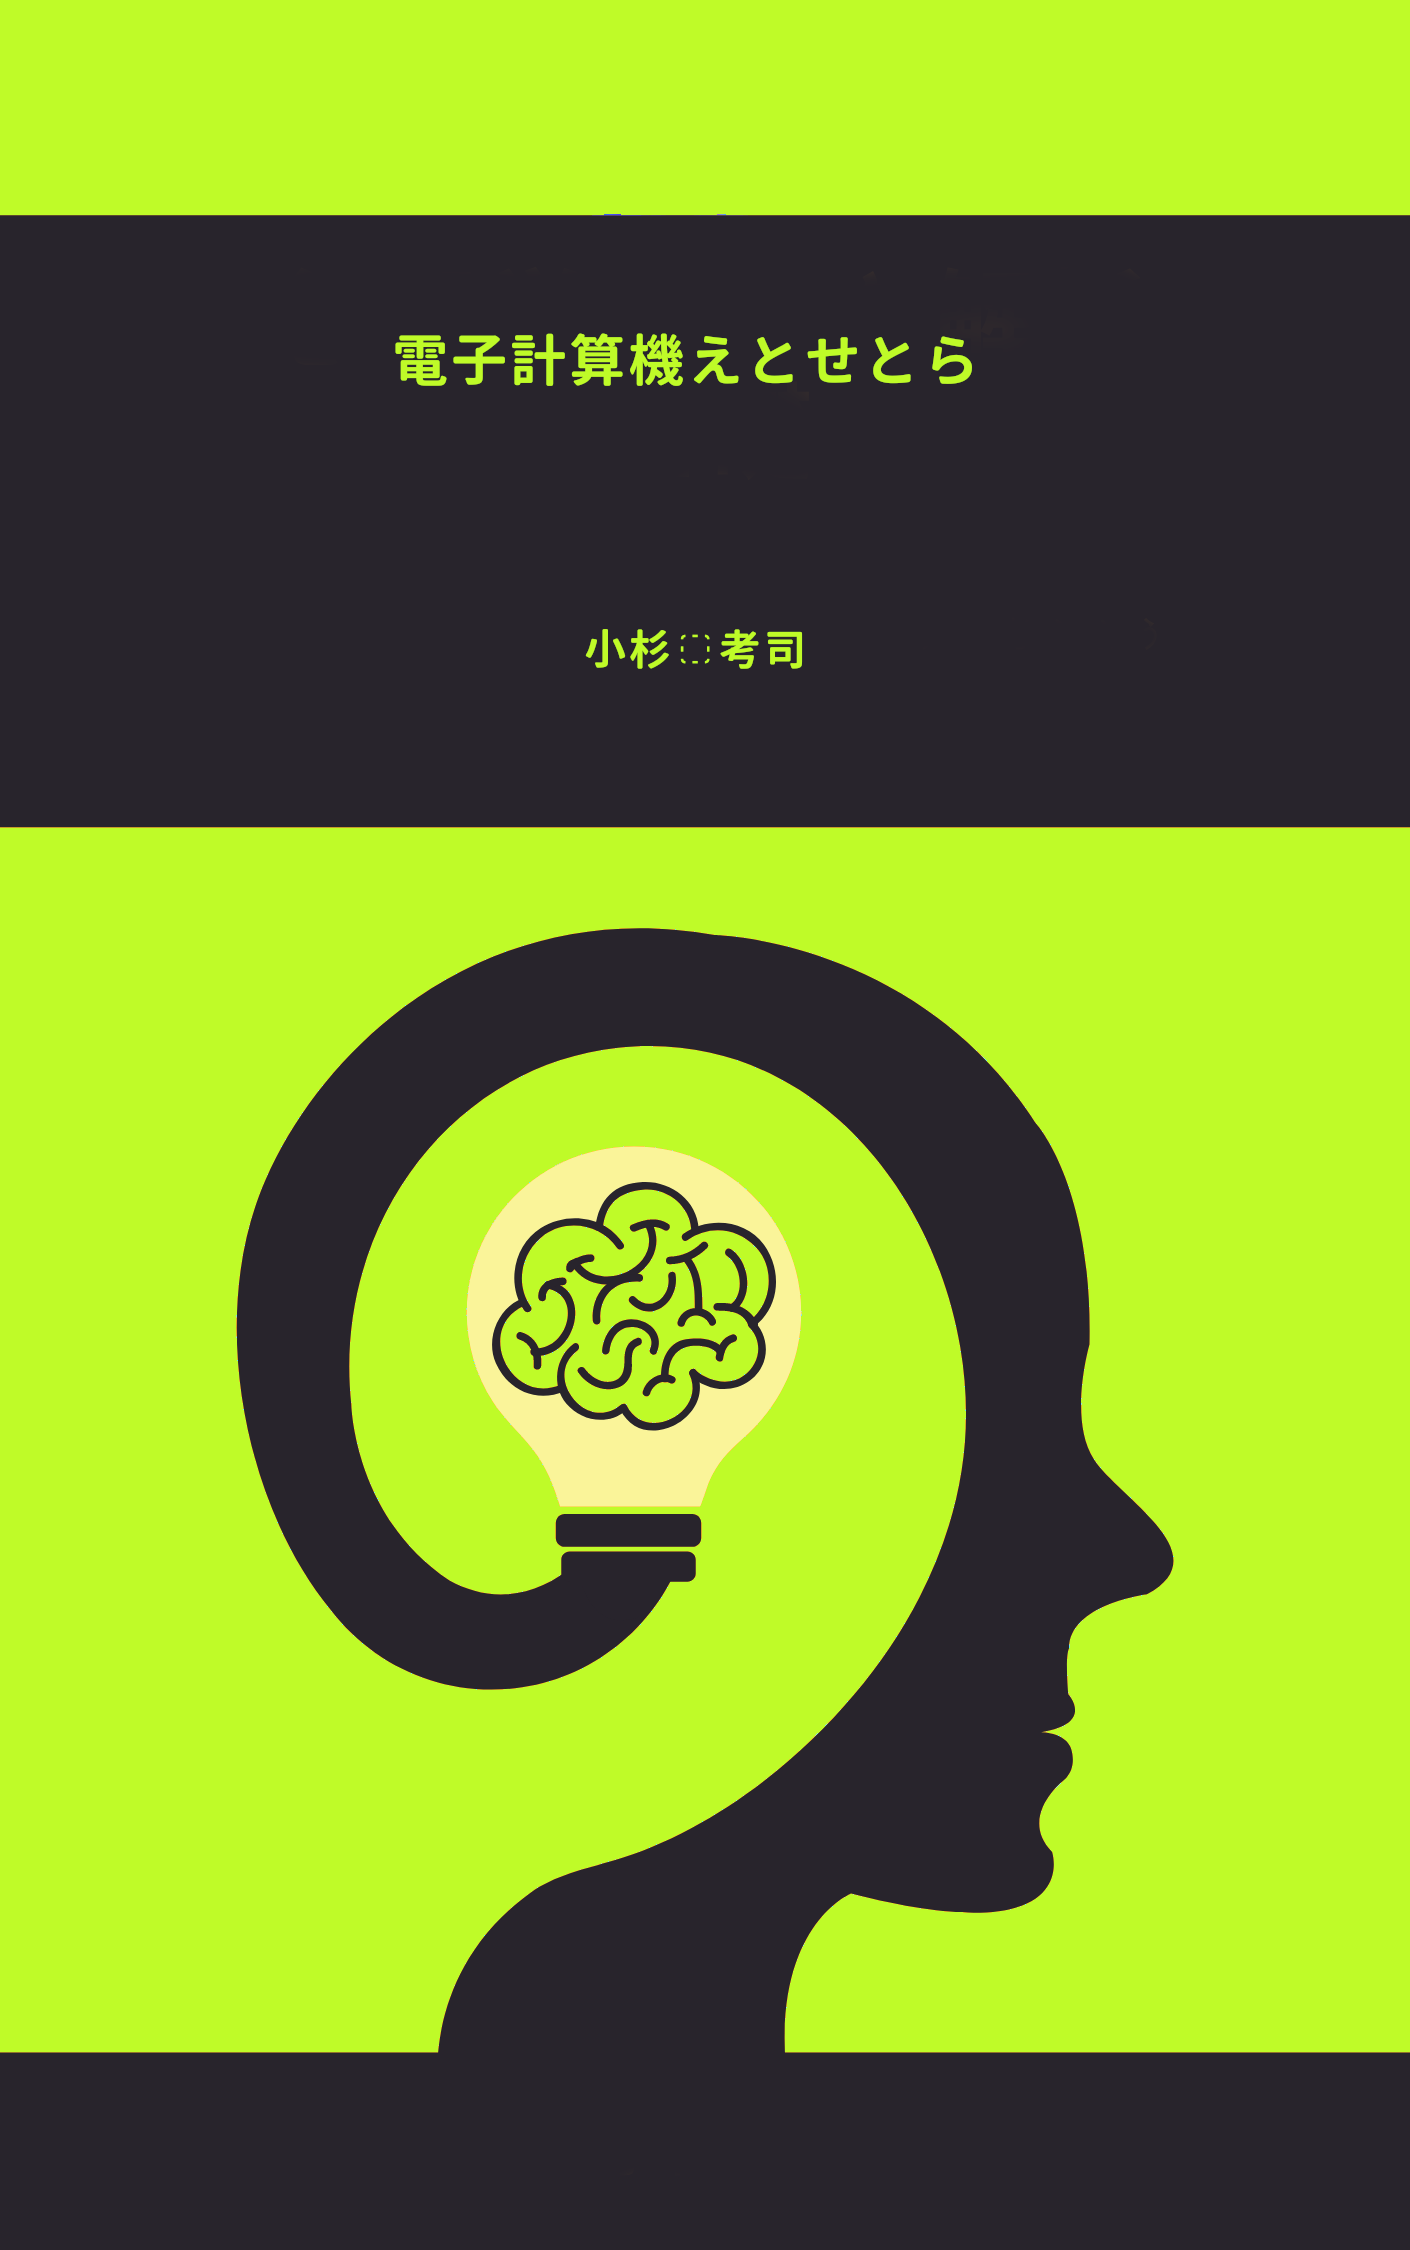
\includepdf[noautoscale=false,pages=-]{Common.png}
\VerbatimFootnotes
% !TEX root = ../pdf/lsj.tex
% [There are multiple lsj.tex files, but the one in ../pdf is the usual one]


\clearpage
\newpage

\vspace*{40pt}

\begin{center}
	この本はCreative Commons BY-SA(CC BY-SA)ライセンスVersion 4.0に基づいて提供されています。著者に適切なクレジットを与える限り，この本を再利用，再編集，保持，改訂，再頒布(商用利用を含む)をすることができます。もし再編集したり，このオープンなテキストを変更したい場合，すべてのバージョンにわたってこれと同じライセンス，CC BY-SA を適用しなければなりません。

	\url{https://creativecommons.org/licenses/by-sa/4.0/deed.ja}

	\vspace*{10pt}

	This book is published under a Creative Commons BY-SA license (CC BY-SA) version 4.0. This means that this book can be reused, remixed, retained, revised and redistributed (including commercially) as long as appropriate credit is given to the authors. If you remix, or modify the original version of this open textbook, you must redistribute all versions of this open textbook under the same license - CC BY-SA.

	\vspace*{18pt}

	\url{https://creativecommons.org/licenses/by-sa/4.0/}
\end{center}

\newpage % copyright page
\title{電子計算機えとせとら}
\author{小杉　考司}
\date{Last Compiled on \number\year .\number\month .\number\day}
\maketitle
\setcounter{tocdepth}{1}

こちらは心理統計教育教材のサイト(\url{https://kosugitti.github.io/psychometrics_syllabus/})で提供されているテキストに共通してつけられる「付録」です。

パソコンなどの電子計算機は，統計を学ぶ時の強力なパートナーであり，基本的な文房具の一種です。
筆者は1976年の生まれですから，まだパソコンのことを「マイコン」と呼んでいた時代からの付き合いです。1980年代の電子計算機は，今から考えると本当に冗談のような演算力，記憶力でした。
その発展のスピードは目覚ましく，最近パソコンを触り始めた人にとっては，スマートフォンやタブレットに比べてパソコンは不便で難しいものに映るかもしれません。
これは少し悲しい話で，最近はどんどん初心者にわかりやすくしようとするあまり，その内部で何が行われているかを隠すことになってしまっているからです。しっかり理解して使うためには，歴史的な経緯やその内部で何が行われているかについて，概略でもいいので知っておく必要があります。そして得てしてその手の知識は，知っている人からしたら「何を今更」というような内容なので，教えるモチベーションもノウハウも育たないのです。

この資料は，筆者のくだらない思い出話も多々含まれていますが，キーボード配列やギリシア文字の読み方といった，周辺知識からなっています。
補助教材としてご利用いただければと思います。

\begin{flushright}
	\date{\today}\\
	小杉考司
\end{flushright}


\tableofcontents


\input{../Computer}
\documentclass{ltjsbook}
\usepackage{docmute} 
\usepackage{../myStyle} 

\begin{document}
\VerbatimFootnotes
\chapter{ギリシア文字一覧}
\label{Greeks}
ギリシア文字ってかっこいいけど，読み方わからない・・・という人のための一覧。ついでに\TeX 表記も。
\begin{table}[ht]
	\centering
	\caption{ギリシア文字とその読み方}
	\begin{tabular}{ccccl}
		読み方   & 大文字           & 小文字          & 英語表記    & \TeX 表記            \\\hline
		アルファ  & $\mathrm{A} $ & \alpha       & alpha   & \verb|\alpha|      \\
		ベータ   & $\mathrm{B}$  & \beta        & beta    & \verb|\beta|       \\
		ガンマ   & \Gamma        & \gamma       & gamma   & \verb|\gamma|      \\
		デルタ   & \Delta        & \delta       & delta   & \verb|\delta|      \\
		エプシロン & $\mathrm{E}$  & \varepsilon  & epsilon & \verb|\varepsilon| \\
		ゼータ   & $\mathrm{Z}$  & \zeta        & zeta    & \verb|\zeta|       \\
		イータ   & $\mathrm{H}$  & \eta         & eta     & \verb|\eta|        \\
		シータ   & \Theta        & \theta       & theta   & \verb|\theta|      \\
		イオタ   & $\mathrm{I}$  & \iota        & iota    & \verb|\iota|       \\
		カッパ   & $\mathrm{K}$  & \kappa       & kappa   & \verb|\kappa|      \\
		ラムダ   & \Lambda       & \lambda      & lambda  & \verb|\lambda|     \\
		ミュー   & $\mathrm{M}$  & \mu          & mu      & \verb|\mu|         \\
		ニュー   & $\mathrm{N}$  & \nu          & nu      & \verb|\nu|         \\
		クサイ   & \Xi           & \xi          & xi      & \verb|\xi|         \\
		オミクロン & $\mathrm{O}$  & $\mathrm{o}$ & omicron & \verb|\mathrm{o}|  \\
		パイ    & \Pi           & \pi          & pi      & \verb|\pi|         \\
		ロー    & $\mathrm{R}$  & \rho         & rho     & \verb|\rho|        \\
		シグマ   & \Sigma        & \sigma       & sigma   & \verb|\sigma|      \\
		タウ    & $\mathrm{T}$  & \tau         & tau     & \verb|\tau|        \\
		ウプシロン & $\mathrm{U}$  & \upsilon     & upsilon & \verb|\upsilon|    \\
		ファイ   & \Phi          & \phi         & phi     & \verb|\phi|        \\
		カイ    & $\mathrm{X}$  & \chi         & chi     & \verb|\chi|        \\
		プサイ   & \Psi          & \psi         & psi     & \verb|\psi|        \\
		オメガ   & \Omega        & \omega       & omega   & \verb|\omega|      \\\hline
	\end{tabular}
\end{table}

\end{document}
\documentclass{ltjsbook}
\usepackage{docmute} 
\usepackage{../myStyle} 

\begin{document}
\VerbatimFootnotes
\chapter{記号の入力とキーボードの場所}
\label{signs}
プログラミングのミスでよくあるのが打ち間違い，スペルミスです。Xとx，Sとsなど大文字と小文字で形が同じものや，l(エルの小文字)と1(数字のイチ)の違いなどは，プログラミング用フォントにして違いがわかるようにするとか，文字列の意味から類推する(Normalとあればノーマルであって，ノーマ・イチではないと察する)など工夫が必要かもしれません。

また，理由はよくわからないのですが頻発するスペルミスは，データ(data)をデート(date)と書いてしまうことです。データはラテン語のdatum(与えられたもの)の複数形なのですが，最近のデータサイエンスの文脈ではdataも単数形と考えるようです。ともかく，日付を表すdateとは由来も意味もスペルも全て違うので，気をつけましょう。

さて，これらはまだ序の口。プログラミングのコードを読んでも，日本語の五十音に入っていない記号の違いがわからない，どこでそれが入力できるかわからない，質問しようにも読み方がわからないといったものもあります。ここではこれらをまとめて解説します。記号の上では微妙な違いですが，当然形が違うのでプログラミング上は違う文字として扱われますので，形の細部までよくみてください。なお，プログラミングでつ変わる時は言語に依存することもありますので，ご注意ください\footnote{たとえばコメントアウトはC言語では\verb|\\|，Rでは\verb|#|，TeXでは\verb|%|など，それぞれ異なります。}。

特に目立つのはハイフンとチルダ，アンダースコアの入力ミスです。それぞれ文字を書く領域における位置が違ったり，形が違ったりするのでよくみてください。
\begin{center}

	\Large{
		\begin{tabular}{ll}
			ハイフンは真ん中  & \verb|A-B| \\
			アンダースコアは下 & \verb|A_B| \\
			オーバーバーは上  & \verb|A¯B| \\
			チルダはニョロ   & \verb|A~B| \\
		\end{tabular}
	}

\end{center}

これを踏まえて，そのほかの記号の名称や意味を表\ref{keyboardName}で確認しましょう。
\begin{table}[ht]
	\centering
	\caption{記号と読み方}
	\label{keyboardName}
	\begin{tabular}{ccl}
		記号        & 読み方            & 解説                                                                         \\\hline
		:         & コロン            & 英文中では「すなわち」などの意味。セミコロンと間違えないように                                            \\
		;         & セミコロン          & 英文中では文章の区切り，接続詞のようにつかう                                                     \\
		.         & ピリオド           & 英文の終わりを意味する。日本語で言う句点                                                       \\
		,         & カンマ            & 英文の区切りを意味する。日本語で言う読点                                                       \\
		\verb|@|  & アットマーク         & メールアドレスに用いられることで有名                                                         \\
		\verb|$|  & ドルマーク          & 米国の通貨単位。Rでは変数名指定のときにもちいる                                                   \\
		/         & スラッシュ          & 割り算の記号                                                                     \\
		*         & アスタリスク         & 掛け算の記号                                                                     \\
		+         & プラス            & 足し算の記号                                                                     \\
		-         & マイナス           & 引き算の記号                                                                     \\
		\verb|^|  & ハット            & 累乗の計算の記号                                                                   \\
		=         & イコール           & 等号。プログラミングでは\verb|==|で一致しているかどうかの判定にも                                      \\
		!         & エクスクラメーション     & 強調。プログラミングでは否定(NOT)の意味になることも                                               \\
		\verb|_|  & アンダースコア，アンダーバー & \begin{tabular}{l}位置に注意。ハイフンではなく文字領域の下の線 \\
			                                                   変数名をつなげる時(ex. \verb|snake_case|)に使ったりする\end{tabular} \\
		\verb|~|  & チルダ            & \begin{tabular}{l}Rでは独立変数と従属変数をつなぐときに使う \\
			                                                   ハイフンやオーバーライン，アンダースコアと間違えられる率高め\end{tabular}          \\
		\verb|¯|  & オーバーライン，オーバーバー & アンダースコアの逆。滅多に使わないが。文字化けを直したときにみられる。                                        \\
		\verb|%|  & パーセント          & プログラミングではコメントアウトの時などに使われたりする                                               \\
		\verb|&|  & アンパサンド         & プログラミングにおけるAND(論理積)の記号など                                                   \\
		\verb|||  & 縦棒             & プログラミングにおけるOR(論理和)，条件付き確率の記号にも                                             \\
		\verb|\|  & バックスラッシュ       & プログラミングではコメントアウトの時などに使われたりする                                               \\
		\verb|"|  & ダブルクォーテーション    & 文字列の開始・終了を表す。同じ記号で閉じる                                                      \\
		\verb|'|  & シングルクォーテーション   & 文字列の開始・終了を表す。同じ記号で閉じる                                                      \\
		\verb|`|  & バッククォーテーション    & 文字列の開始・終了を表す。同じ記号で閉じる                                                      \\
		\verb|[]| & 大括弧            & プログラミングでは配列を意味することがある                                                      \\
		\verb|{}| & 中括弧            & プログラミングではブロックの開始と終了を意味することがある                                              \\
		\verb|()| & 小括弧            & 数式のまとまりを表す                                                                 \\\hline
	\end{tabular}
\end{table}


一般的な日本語キー配列の場合，1つのキーに4つの文字・記号が割り当てられていますが，英語入力モードの場合はキーの左側，日本語入力モードはキーの右側を見ることになります。キーを押すと下の段の文字が入力されますが，シフトキーを押しながらキーを押すことで上の段の文字が入力されることになります(図\ref{JPkeyChange})。

これを踏まえて，日本語キーについては\ref{jpKeyAssign}，USキーについては図\ref{usKeyAssign}に代表的な記号とキー配列の位置を示しました。入力に困った場合は一度図を見て確認してください\footnote{USキー配列はキートップに一種類の文字しかなく，美しい配置なのでおすすめです。}。
\begin{figure}[ht]
	\centering
	
\includegraphics[keepaspectratio,width=4cm]{../common_contents/figures/JapaneseKeyChange.png}
	\caption{日本語キーで入力する場合}
	\label{JPkeyChange}
\end{figure}
\begin{figure}[ht]
	\centering
	
\includegraphics[keepaspectratio,width=0.8\linewidth]{../common_contents/figures/JPkeyAssign.png}
	\caption{代表的な記号と日本語キー配列}
	\label{jpKeyAssign}
\end{figure}
\begin{figure}[ht]
	\centering
	
\includegraphics[keepaspectratio,width=0.8\linewidth]{../common_contents/figures/usKeyAssign.png}
	\caption{代表的な記号とUSキー配列}
	\label{usKeyAssign}
\end{figure}

\end{document}


\addcontentsline{toc}{chapter}{引用文献}
% 引用文献
\printbibliography[title=引用文献]
% 索引
\addcontentsline{toc}{chapter}{索引}

\printindex
\end{document}